\subsection{Retrieval Augmented Generation}
Se conoce como \aclink{RAG} a la arquitectura que combina la recuperación de información con la generación de texto. Esta arquitectura se compone de dos partes principales: un modelo de recuperación y un modelo de generación. El modelo de recuperación se encarga de recuperar información relevante de una base de conocimiento, mientras que el modelo de generación se encarga de generar texto basado en la información recuperada.

Esta arquitectura es especialmente útil cuando se trabaja con modelos de lenguaje grandes, ya que mejora el problema de las alucinaciones. En lugar de generar respuestas en base al conocimiento del que disponen durante el entrenamiento, que puede dar resultados erróneos, el modelo puede acceder a bases de conocimiento factual con las que puede generar respuestas más precisas y acordes al contexto.

\subsubsection{Funcionamiento}
El funcionamiento típico de esta arquitectura consta de un flujo dividido en dos partes principales, la recuperación de contexto y la generación de respuestas, que se explicarán brevemente a continuación:

Durante la recuperación de contexto se consulta en una base de conocimiento, que podría ser una base de datos vectorial, un grafo de conocimiento o una ontología, entre otros. Para hacer una consulta, se ha de contrastar la pregunta que un usuario haga con la información contenida, para obtener la información más relevante posible. Esta tarea requiere gran atención ya que es crucial de cara al desempeño que vaya a lograr el sistema.

Una vez se ha recuperado la información, se pasa a la generación de respuestas. En esta etapa, se utiliza la información recuperada junto con la pregunta inicial para guiar al modelo de lenguaje en la generación de respuestas. De esta manera, el modelo puede generar respuestas más precisas y acordes al contexto proporcionado.

\begin{figure}[!h]
    \centering
    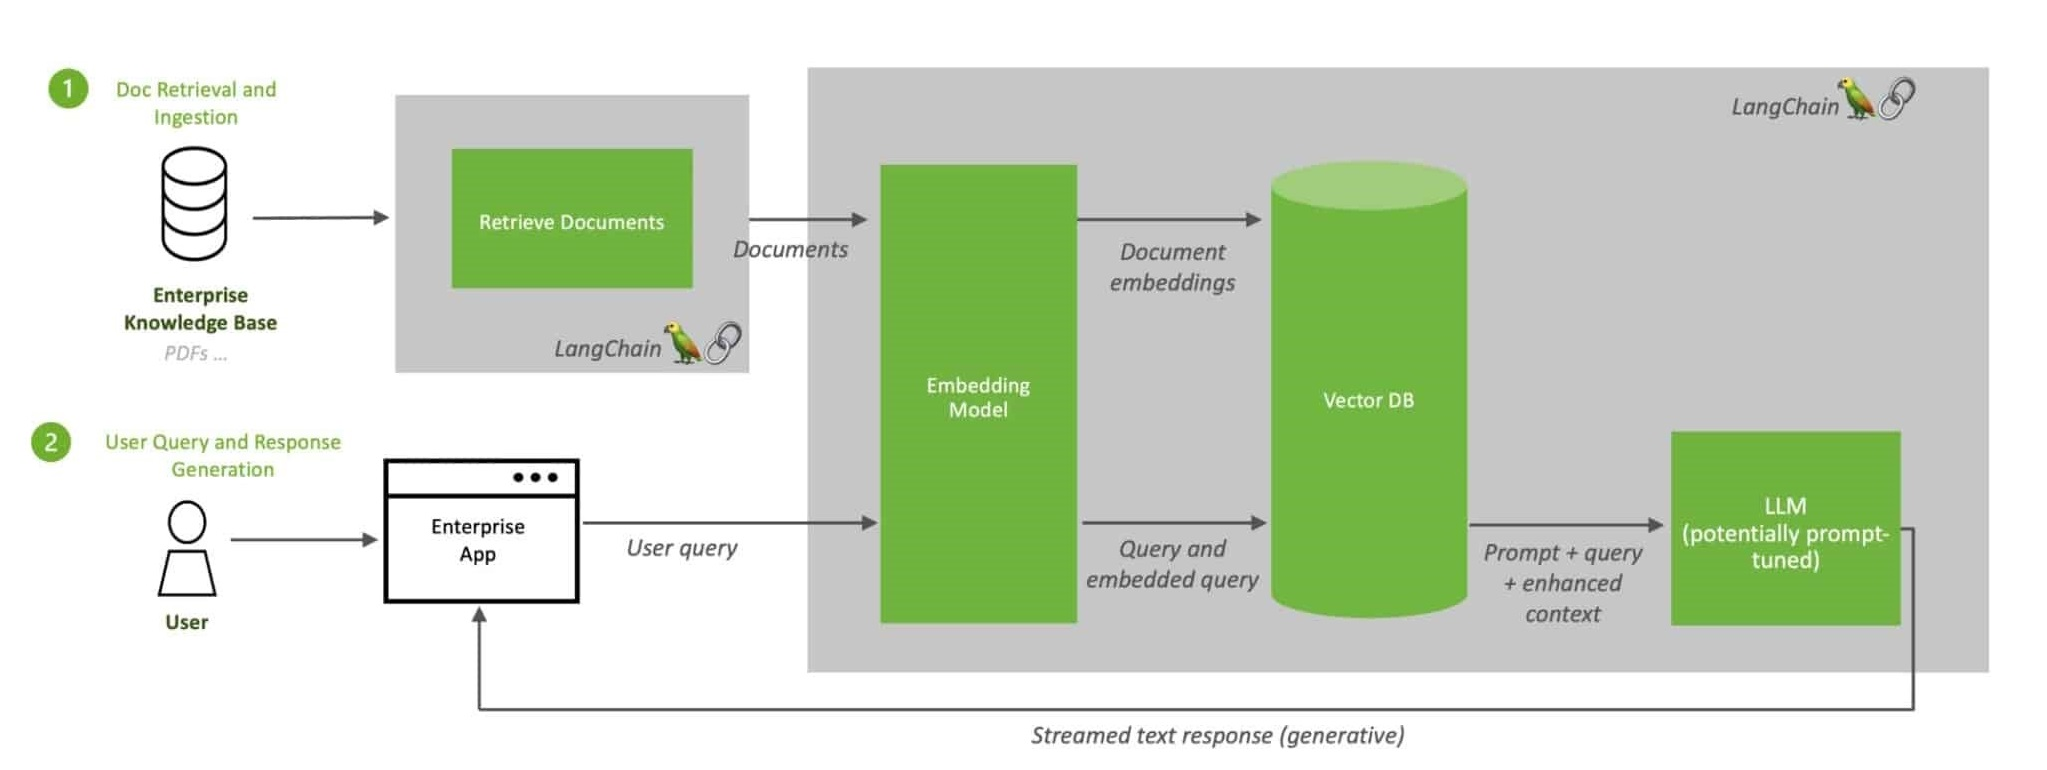
\includegraphics[width=0.8\textwidth]{images/rag.jpg}
    \caption{Esquema de funcionamiento de una arquitectura RAG~\cite{nvidiaBlog}}
    \label{fig:rag}
\end{figure}